\documentclass[11pt]{article}
\usepackage[scaled=0.92]{helvet}
\usepackage{geometry}
\geometry{letterpaper,tmargin=1in,bmargin=1in,lmargin=1in,rmargin=1in}
\usepackage[parfill]{parskip} % Activate to begin paragraphs with an empty line rather than an indent %\usepackage{graphicx}
\usepackage{amsmath,amssymb, mathrsfs, dsfont}
\usepackage{tabularx}
\usepackage[font=footnotesize,labelfont=bf]{caption}
\usepackage{graphicx}
\usepackage{xcolor}
%\usepackage[linkbordercolor ={1 1 1} ]{hyperref}
%\usepackage[sf]{titlesec}
\usepackage{natbib}
\usepackage{../../Tianpei_Report}

%\usepackage{appendix}
%\usepackage{algorithm}
%\usepackage{algorithmic}

%\renewcommand{\algorithmicrequire}{\textbf{Input:}}
%\renewcommand{\algorithmicensure}{\textbf{Output:}}



\begin{document}
\title{Lecture 1: Fundamental of Curves and Surface in $\bR^{3}$}
\author{ Tianpei Xie}
\date{ Jun. 1st., 2015 }
\maketitle
\tableofcontents
\newpage
\section{Curves}
\subsection{Regular Curves in $\bR^3$}
\begin{itemize}
\item \begin{definition}
A \emph{\textbf{parameterized differentiable curve}} \citep{do1976differential} is a differentiable map $\alpha: I \rightarrow \bR^{3}$ of an open interval $I = (a,b) \subset \bR$ to $\bR^{3}$. 
\end{definition}

The word \emph{differentiable} in this definition means that $\alpha$ is a correspondence which maps each $t \in I$ into a point $\alpha(t) = (x(t), y(t), z(t)) \in \bR^3$ in such a way that the functions $x(t)$, $y(t)$, $z(t)$ are differentiable. The variable $t$ is called the \emph{parameter of the curve}. The word interval is taken in a generalized sense, so that we do not exclude the cases $a = -\infty$, $b = +\infty$.

If we denote by $x'(t)$ the first derivative of $x$ at the point $t$ and use similar notations for the functions $y$ and $z$, the vector $(x'(t), y'(t), z'(t)) = \alpha'(t) \in \bR^3$ is called the \emph{\textbf{tangent vector}} (or velocity vector) of the curve $\alpha$ at $t$. The image set $\alpha(I) \subset \bR^3$ is called the \emph{trace} of $\alpha$. 

\item \begin{definition}
A parameterized curve is said to be \emph{\textbf{regular}} if $\alpha'(t)\neq 0$ for all $t\in I$.
\end{definition}

\item The \emph{arc length} of a regular parameterized curve $\alpha: I \rightarrow \bR^{3}$ from $t_{0}$ is defined as
\begin{align*}
s &\equiv \int_{t_{0}}^{t}\abs{\alpha'(t)} dt 
\end{align*} where $\abs{\alpha'(t)} = \sqrt{(x'(t))^{2} + (y'(t))^{2}+ (z'(t))^{2}}$. Note that a parameterized regular curve can be reparameterized by the arc length as $\alpha(s)$.

\item Given the curve $\alpha$ parametrized by arc length $s \in (a, b)$, we may consider the curve $\beta$ defined in $(-b, -a)$ by $\beta(-s) = \alpha(s)$, which has the same trace as the first one but is described in the \emph{opposite direction}. We say, then, that these two curves differ by \emph{\textbf{a change of orientation}}.
\end{itemize}



\subsection{Vector Product in $\bR^3$}
\begin{itemize}
\item Two ordered bases $e = [e_i]$ and $f = [f_i]$, $i = 1,\ldots,n$, of an $n$-dimensional vector space $V$ have \emph{t\textbf{he same orientation}} if the matrix of change of basis has positive determinant. We denote this relation by $e \sim f$. From elementary properties of determinants, it follows that $e \sim f$ is an \emph{\textbf{equivalence relation}}.

\item Each of the equivalence classes determined by the above relation is called an \emph{\textbf{orientation}} of $V$.

\item In the case $V = \bR^3$, there exists a natural ordered basis $e_1 = (1, 0, 0)$, $e_2 = (0, 1, 0)$, $e_3 = (0, 0, 1)$, and we shall call the orientation corresponding to this basis the \emph{\textbf{positive orientation}} of $\bR^3$, the other one being the \emph{negative orientation} (of course, this applies equally well to any $\bR^n$). 

We also say that \emph{\textbf{a given ordered basis}} of $\bR^3$ is \emph{\textbf{positive (or negative)}} if it belongs to the positive (or negative) orientation of $\bR^3$. Thus, the ordered basis $e_1, e_3, e_2$ is a negative basis,since the matrix which changes this basis into $e_1,e_2,e_3$ has determinant equal to $-1$.

\item The \emph{\textbf{cross product}} (\emph{\textbf{vector product}}) of two vectors $u$ and $v$ under the basis $\set{e_{1}, e_{2}, e_{3}}$ is denoted as $u\wedge v$ and computed as
\begin{align}
\inn{u\wedge v}{w} &= \det\abs{\begin{array}{ccc}
u_{1} & u_{2} & u_{3} \\ 
v_{1} & v_{2} & v_{3} \\ 
w_{1} & w_{2} & w_{3}
\end{array} }  \equiv \det(u, v, w)\label{eqn: cross_prod}
\end{align}
and
\begin{align}
u\wedge v \equiv u \times v &\equiv \abs{\begin{array}{cc}
u_{2} & u_{3} \\ 
v_{2} & v_{3}
\end{array} }e_{1}
- 
\abs{\begin{array}{cc}
u_{1} & u_{3} \\ 
v_{1} & v_{3}
\end{array} }e_{2}
+
\abs{\begin{array}{cc}
u_{1} & u_{2} \\ 
v_{1} & v_{2}
\end{array} }e_{3}  \label{eqn: cross_prod2}
\end{align}

\item The following \textbf{properties} can easily be checked (actually they just express
the usual \emph{properties of \textbf{determinants}}):
\begin{enumerate}
\item (\textbf{\emph{anti-commutativity}}) $u \wedge v = - v \wedge u$.
\item $u \wedge v$ depends \emph{\textbf{linearly}} on $u$ and $v$; i.e., for any real numbers $a$, $b$, we have
$(a\,u+b\,w) \wedge v = a\,(u \wedge v)+b\,(w \wedge v)$.
\item $u \wedge v = 0$ if and only if $u$ and $v$ are \emph{\textbf{linearly dependent}}.
\item $\inn{u \wedge v}{u} = 0$, $\inn{u \wedge v}{v} = 0$.
\end{enumerate}

\item We observe that $\inn{u \wedge v}{u \wedge v} = \abs{u \wedge v}^2 > 0$. This means that the determinant of the vectors $u$, $v$, $u \wedge v$ is \emph{positive}; that is, \emph{\textbf{$\set{u, v, u \wedge v}$ is a positive basis}} (Figure \ref{fig: cross_product_basis}).

\begin{figure}[tb]
\begin{minipage}{1\linewidth}
 \centerline{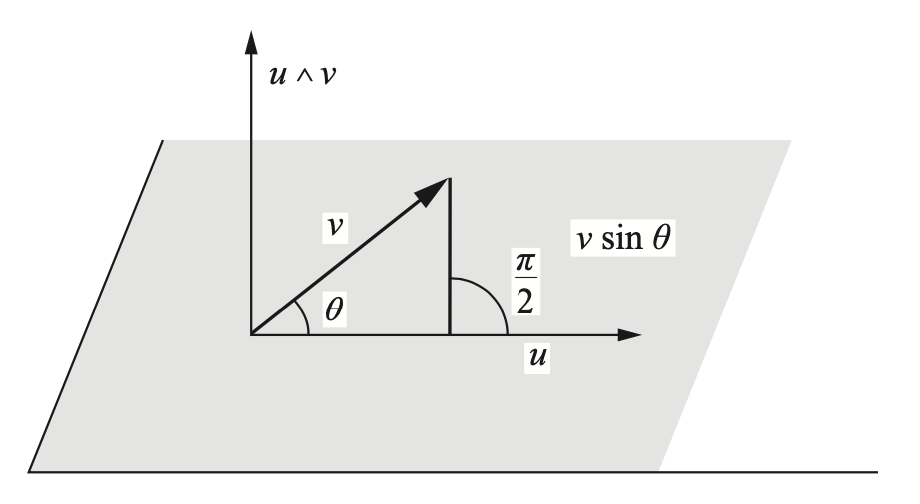
\includegraphics[scale = 0.5]{cross_product_basis.png}}
\end{minipage}
\caption{\scriptsize\textbf{The basis of $\bR^3$ formed by $u, v, u \wedge v$ \citep{do1976differential}}}
\label{fig: cross_product_basis}
\end{figure}

\item The inner product of vector products is 
\begin{align*}
\inn{u\wedge v}{x \wedge y} &= \det\brac{\begin{array}{cc}
\inn{u}{x} & \inn{u}{y}  \\ 
\inn{v}{x} & \inn{v}{y} 
\end{array} }
\end{align*}
It follows that 
\begin{align*}
\inn{u\wedge v}{u \wedge v} = \abs{u \wedge v}^2  &= \det\brac{\begin{array}{cc}
\inn{u}{u} & \inn{u}{v}  \\ 
\inn{v}{u} & \inn{v}{v} 
\end{array} } = \abs{u}^2\abs{v}^2\,(1- \cos^2(\theta)) = A^2
\end{align*} where $\theta$ is the \emph{\textbf{angle}} of $u$ and $v$, and $A$ is the \emph{\textbf{area}} of the \emph{\textbf{parallelogram}} generated by $u$ and $v$.

\item Note that the vector product is \textbf{not associative}. In fact, we have the following identity:
\begin{align}
(u \wedge v) \wedge w &= (\inn{u}{w})\,v - (\inn{v}{w})\,u. \label{eqn: cross_prod_cros_prod_again}
\end{align}

\item Finally, let $u(t) = (u_1(t), u_2(t), u_3(t))$ and $v(t) = (v_1(t), v_2(t), v_3(t))$ be differentiable maps from the interval $(a, b)$ to $\bR^3$, $t \in (a, b)$. It follows immediately from Eq. \eqref{eqn: cross_prod2} that $u(t) \wedge v(t)$ is also differentiable and that
\begin{align*}
\frac{d}{dt}(u(t) \wedge v(t)) &= \frac{d u(t)}{dt} \wedge v(t) + u(t) \wedge \frac{d v(t)}{dt}
\end{align*}

\end{itemize}

\subsection{The Local Theory of Curves Parametrized by Arc Length}
\begin{itemize}
\item The differential of $\alpha(s)$ as $t(s) \equiv \overrightarrow{t}(s) \equiv \alpha'(s)$ is the \emph{\textbf{tangent vector}} (velocity) of $\alpha(s)$ at $s$. 

\item 
\begin{definition}
The quantity $\abs{\alpha''(s)} \equiv k(s)$ is referred as the \emph{\textbf{curvature}} of $\alpha(s)$ at $s$. The curvature measures \emph{\textbf{the rate of change}} of \emph{the tangent line} along the curve. 
\end{definition}

Notice that by a change of orientation, the tangent vector changes its direction; that is, if $\beta(-s) = \alpha(s)$, then
\begin{align*}
\frac{d \beta(-s)}{d(-s)} &= -\frac{d\alpha(s)}{ds}
\end{align*}

Therefore, $\alpha''(s)$ and the curvature remain \emph{\textbf{invariant}} under \emph{a change of orientation}.

\item For any \textbf{\emph{closed}} parameterized \textbf{\emph{convex}} curve, the curvature $k(s)$ is \textbf{nonnegative} and has \textbf{two} maxima and \textbf{two} minima or is constant everywhere. 

\item Moreover, the acceleration vector  $\alpha''(s)$ is \emph{\textbf{normal}} (orthogonal) to $\alpha'(s)$, because by differentiating $\inn{\alpha'(s)}{\alpha'(s)} = 1$ we obtain $\inn{\alpha''(s)}{\alpha'(s)} = 0$. 

Let $n(s)$ be the unit vector of $\alpha''(s)$ (i.e. $\alpha''(s) = k(s)\,\mb{n}(s)$), then $\mb{n}(s) \equiv \overrightarrow{n}(s)$ is the \emph{\textbf{normal vector}} and it perpendicular to the tangent vector.

\item The plane determined by the unit \emph{tangent} and \emph{normal vectors}, $\alpha'(s)$ and $n(s)$, is called the \emph{\textbf{osculating plane}} at $s$

\begin{figure}[tb]
\begin{minipage}{1\linewidth}
 \centerline{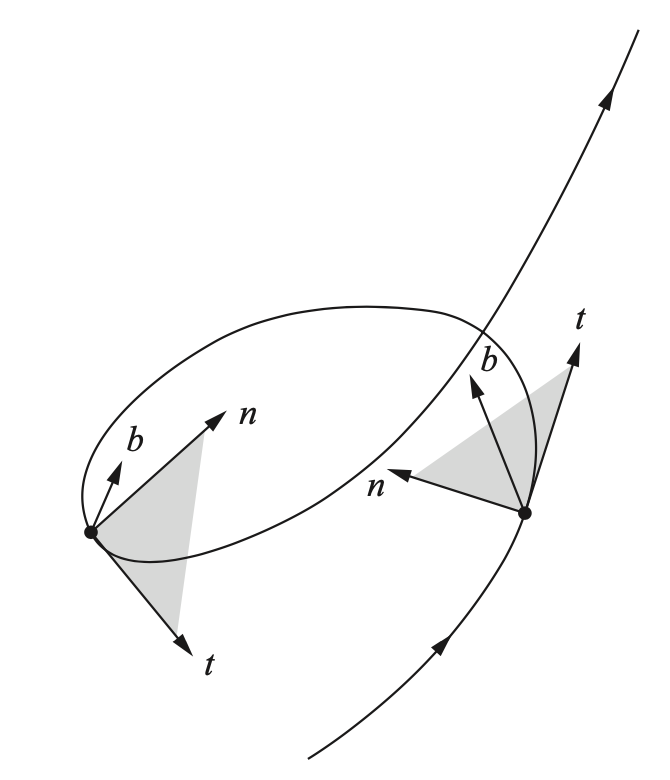
\includegraphics[scale = 0.6]{osculating_plane.png}}
\end{minipage}
\caption{\scriptsize\textbf{The osculating plane spanned by tangent vector $t(s) = \alpha'(s)$ and normal vector $n(s)$ with binormal vector $b(s)$ as its normal vector \citep{do1976differential}}}
\label{fig: osculating_plane}
\end{figure}

\begin{figure}[htb]
\centering
\begin{minipage}{0.6\linewidth}
 \centerline{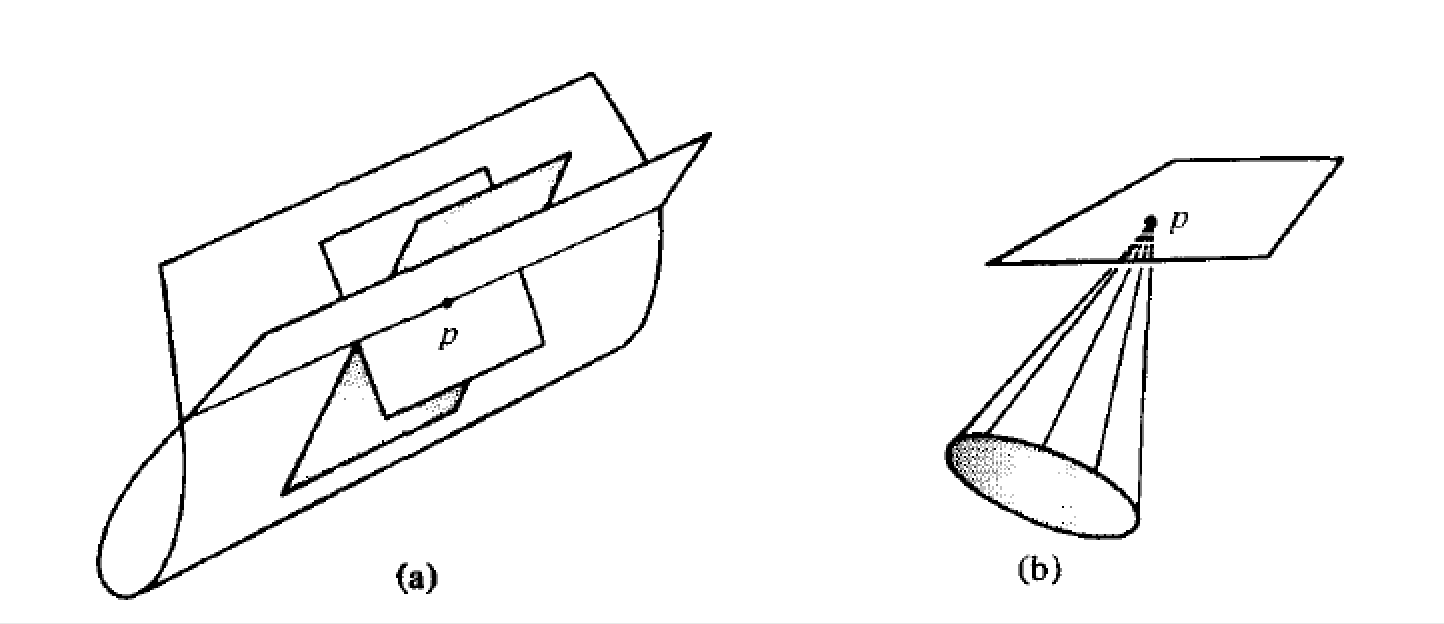
\includegraphics[scale = 0.5]{regular_surface.png}}
\end{minipage}
\caption{\scriptsize{\textbf{The situation avoided in the definition of regularity. (a) When the parameterization is not one-to-one, then the self-intersection of the surfaces will happen;   (b) When the differential is not one-to-one at $p$, thus the tangent plane is not defined uniquely. }}}
\label{fig: regular_surface}
\end{figure}

\item We say that $s \in I$ is a \emph{singular point} of order $1$ if $\alpha''(s) = 0$.

\item Define the vector $b(s) = t(s) \wedge n(s)$ as the \emph{\textbf{binormal vector}}. It is the normal vector of the $t-n$ plane and it is orthogonal to $(t(s), n(s))$. 

\item The differential of binormal vector $b'(s)$ characterize the \emph{\textbf{strength} of the curve} to \emph{\textbf{pull away from the plane}} where it currently lies. Its length $\abs{b'(s)}$ measures the rate of change of the neighboring osculating planes with the osculating plane at $s$.

\item  $b'(s)$ is \emph{\textbf{parallel}} to $n(s)$ and is computed as $b'(s) = \tau(s)\,n(s)$ \citep{do1976differential}. (Some book use $b'(s) = -\tau(s)\,n(s)$. )

\begin{definition}
Let $\alpha: I \rightarrow \bR^3$ be a curve parametrized by arc length $s$ such that $\alpha''(s) \neq 0$, $s \in I$. The number $\tau(s)$ defined by $b'(s) = \tau(s)\,n(s)$ is called the \emph{\textbf{torsion}} of $\alpha(s)$ at $s$.
\end{definition}

\begin{figure}[tb]
\begin{minipage}{0.7\linewidth}
 \centerline{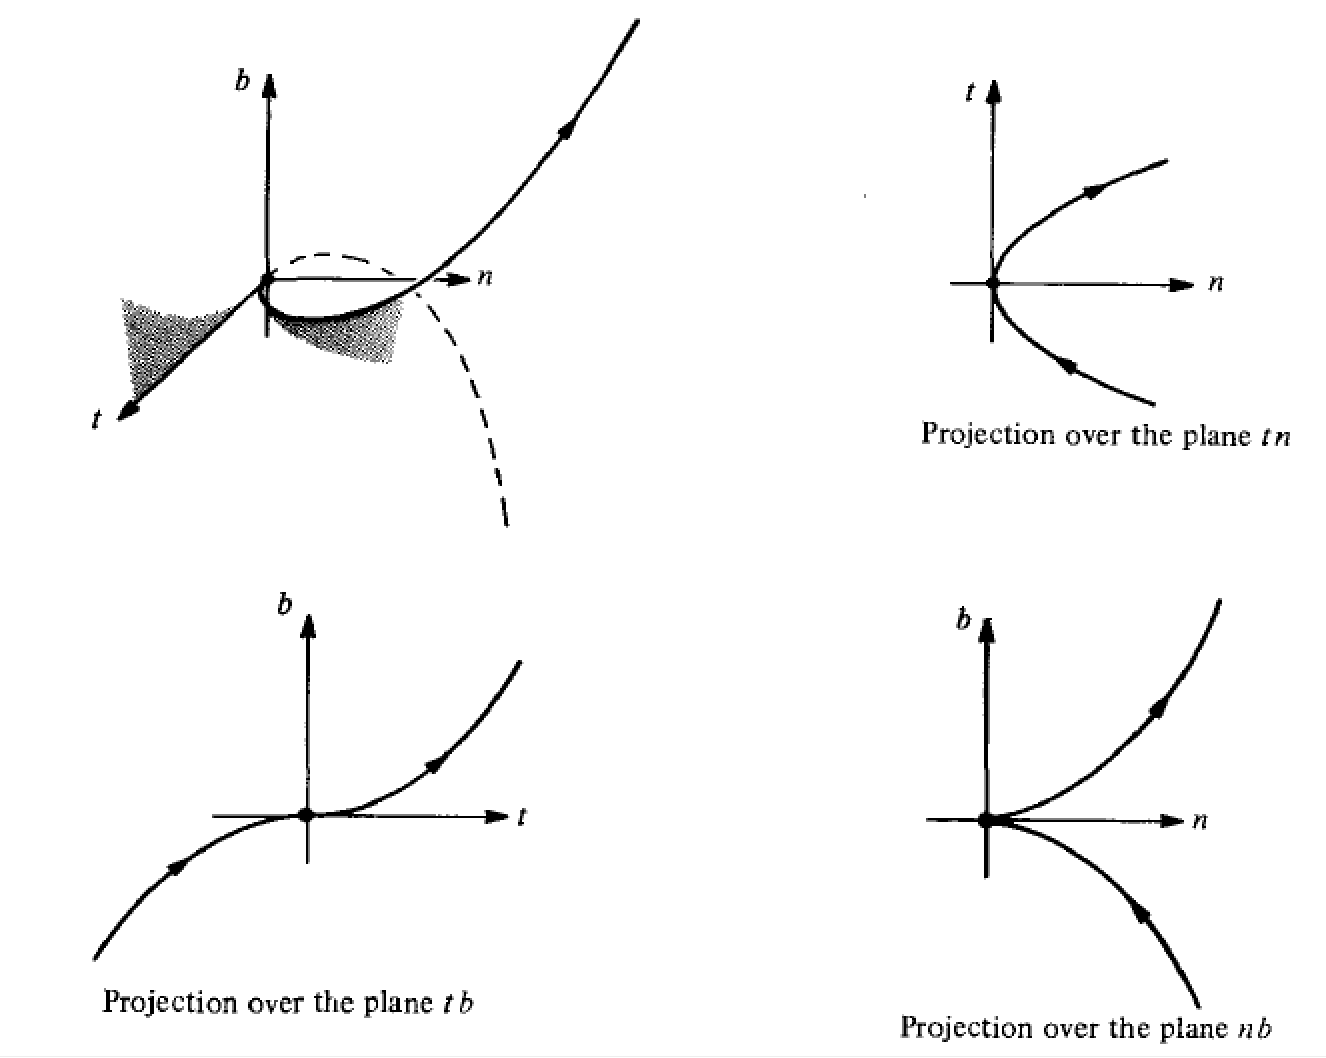
\includegraphics[scale = 0.5]{Frenet_trihedron.png}}
\end{minipage}
\caption{\scriptsize
\textbf{The local behavior of general regular curve. At the osculating plane, it is like a parabola. At the normal plane, it is like a cubic function. }}
\label{fig: Frenet_trihedron}
\end{figure}

If $\tau \equiv 0$, then the \emph{curve will lies \textbf{entirely in a plane}} and vise versa.   Note that $k(s)\neq 0$ is essential for above argument to hold. 

In contrast to the curvature, the torsion may be either positive or negative. The \textbf{sign} of torsion is related to the \emph{\textbf{orientation}} of the curve relative to the \emph{\textbf{osculating plane}}. 

\item Both $k(s)$ and $\tau(s)$ are \emph{\textbf{invariant}} to change of orientation. 

\item The three orthonormal vectors $(t(s), n(s), b(s))$ \textbf{form a basis} that uniquely characterizes the local behavior of a curve, and it is called the \emph{\textbf{Frenet trihedron}} at $s$. The curvature $k$ and the torsion $\tau$ will reveal information of curve $\alpha$ in the neighborhood of $s$.

\item Given $\tau(s)$ and $k(s)$, the curve at $s$ can be reparameterized via the trihedron $(\mb{t}, \mb{n}, \mb{b})$. 

\item The plane spanned by $(t, n)$ is called \emph{\textbf{osculating plane}}. The plane spanned by $(n, b)$ is called \emph{\textbf{normal plane}} and the plane spanned by $(t, b)$ is called \emph{\textbf{rectifying plane}}.

\item The Frenet trihedron $(t, n, b)$ at $s$ can be computed via the \emph{system of differential equations} as 
\begin{align}
t' &= k\,n\nonumber\\
n' &= -k\,t - \tau\,b\nonumber\\
b' &= \tau\,n \label{eqn: Frenet_formula}
\end{align}
called \emph{\textbf{Frenet formula}} \citep{do1976differential}, where $k(s)>0$ and $\tau(s)$ are the curvature and torsion of a regular parameterized curve, respectively.  

From theorem \ref{th: curv_tri}, we see that the curvature and torsion function determine a parameterized regular curve \textbf{up to a rigid transformation}.  It is thus called \emph{the fundamental theorem of the local theory of curves}.

\item 
\begin{theorem}\label{th: curv_tri} 
(\textbf{The fundamental theorem of the local theory of curves})  \citep{do1976differential}\\
Given differentiable functions $k(s)>0$ and $\tau(s)$ for $s\in I$, there exists a regular parameterized curve $\alpha: I\rightarrow \bR^{3}$ such that $s$ is the arc length, $k(s)$ is the curvature and $\tau(s)$ is the torsion. Moreover, any other curve $\hat{\alpha}$ satisfying the conditions above differ from $\alpha$ by a \textbf{rigid transformation} as $\hat{\alpha} = \rho\circ \alpha + c$ for $\rho$ \textbf{an orthogonal transformation} and $c$ \textbf{a translation vector}. 
\end{theorem}\vspace{5pt}
\end{itemize}

\section{Regular Surfaces}
\subsection{Surfaces}
\begin{itemize}
\item
\begin{definition}
 A subset $\cS \subset \bR^{3}$ is a \emph{\textbf{regular surface}} \citep{do1976differential}, if for any $p\in \cS$, there exists a neighborhood $V \subset \bR^{3}$ and a map $\mb{x}: U \subset \mb{R}^{2} \rightarrow V\cap \cS$ of an open subset $U\subset \mb{R}^{2}$ onto $V \cap \cS \subset \bR^{3}$ such that 
\begin{enumerate}
\item $\mb{x}:  (u,v) \in U \rightarrow  (x(u,v), y(u,v), z(u,v))$ has \emph{\textbf{differentials}} in $U$ with all orders. 
\item $\mb{x}$ is a \textbf{\emph{homemorphism}}, i.e. $\mb{x}$ is a \emph{\textbf{continuous bijection}} with \emph{\textbf{continuous inverse}} $\mb{x}^{-1}: W \supset V\cap \cS \rightarrow \bR^{2}$.
\item (\textbf{\emph{The regularity condition}.}) For any $q\in U$, the differential $d\mb{x}_{q}$ is one-to-one, i.e. \emph{\textbf{injective}}.   
\end{enumerate}   
\end{definition}

Let $q = (u_0, v_0)$. The vector $e_1$ is tangent to the curve $u \rightarrow (u, v_0)$ whose image under $\mb{x}$ is the curve
\begin{align*}
u \rightarrow (x(u, v_0), y(u, v_0), z(u, v_0)).
\end{align*} This image curve (called the \emph{coordinate curve} $v = v_0$) lies on $\cS$ and has at $\mb{x}(q)$ the tangent vector
\begin{align*}
\partdiff{\mb{x}}{u} &= \paren{\partdiff{x}{u}, \partdiff{y}{u}, \partdiff{z}{u}}.
\end{align*} where the derivatives are computed at $(u_0,v_0)$ and a vector is indicated by its components in the basis $\set{f_1 , f_2 , f_3 }$. By the definition of differential
\begin{align*}
d\mb{x}_{q}(e_1)\paren{\partdiff{x}{u}, \partdiff{y}{u}, \partdiff{z}{u}} &= \partdiff{\mb{x}}{u}
\end{align*} Similarly, for coordinate curve $u = u_0$, 
\begin{align*}
d\mb{x}_{q}(e_2)\paren{\partdiff{x}{v}, \partdiff{y}{v}, \partdiff{z}{v}} &= \partdiff{\mb{x}}{v}
\end{align*}
Thus
\begin{align*}
dx_{q} \equiv \partdiff{(x,y,z)}{(u,v)} = \brac{\begin{array}{cc}
\partdiff{x}{u} & \partdiff{x}{v} \\
\partdiff{y}{u} & \partdiff{y}{v} \\
\partdiff{z}{u} & \partdiff{z}{v}
\end{array}}
\end{align*}. The condition 3 requires that $\partdiff{(x,y,z)}{(u,v)}$ has full column rank. 

\begin{figure}[htb]
\centering
\begin{minipage}{0.6\linewidth}
 \centerline{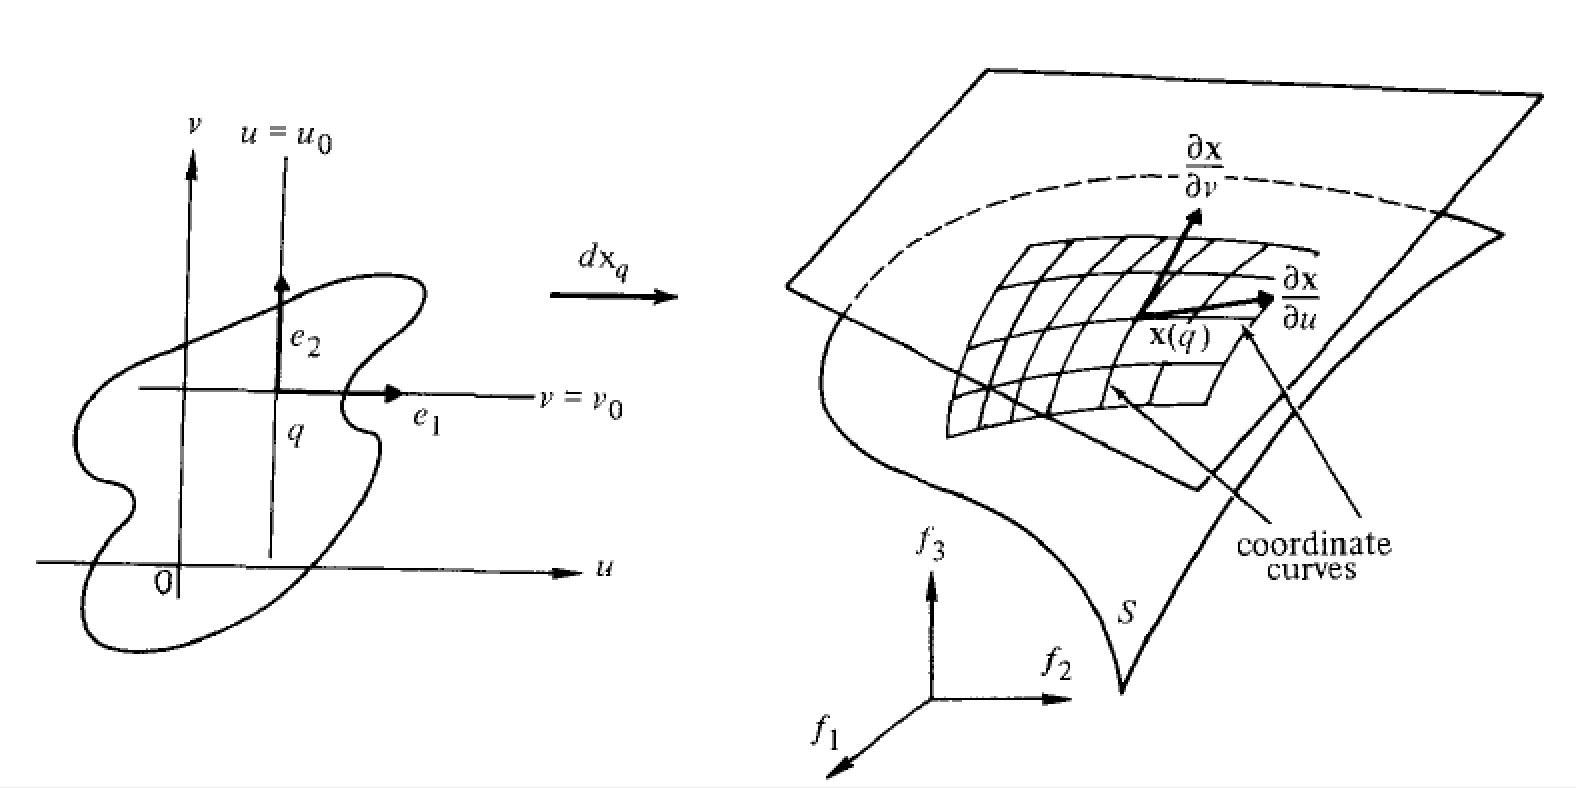
\includegraphics[scale = 0.5]{coordinate_curve.png}}
\end{minipage}
\label{fig: coordinate_curve}
\end{figure}

\item \begin{definition}
The map $\mb{x}: U\subset \bR^{2} \rightarrow V\cap \cS$ is called a \emph{\textbf{parameterization}} of the surface (at $p$). Its inverse $\mb{x}^{-1}: W\supset V\cap \cS \rightarrow U$ is called a \emph{\textbf{coordinate system}}. We may write $\mb{x}^{-1} = (u, v)$, where $u,v$ are smooth function on $W$ and are called \emph{\textbf{coordinate functions}} (\emph{local coordinate} of surface at $p$ as $p= (u,v)$). The neighborhood $V\cap \cS$ of $p$ is called the \emph{coordinate neighborhood} of $p$ in $\cS$. 
\end{definition}

\item \begin{theorem}\label{th: surf_difffun}
If $f: U\subset \bR^{2} \rightarrow \bR$ is a differentiable function in an open set $U$ of $\bR^{2}$, then the graph of $f$, $(u,v, f(u,v))$ is a regular surface in $\bR^{3}$ for $(u,v) \in U$.
\end{theorem}


\item \begin{definition}
Given a differentiable map $F: U\subset \bR^{n} \rightarrow \bR^{m}$, a point $p\in U$ is a \emph{\textbf{critical point}} of $F$ if $dF_{p}$ is not surjective, i.e. $\partdiff{F}{(\xi_{1}, \ldots, \xi_{m})} = \mb{0}$. The image of critical point is a \emph{\textbf{critical value}}. The value $r$ that is not a critical value is called \emph{\textbf{regular value}} of $F$. Note $dF_{q} \neq 0$ for all $q\in F^{-1}(r)$. 
\end{definition}

\item \begin{definition}
For $p$ in a regular surface $\cS$ and let one associated parameterization $\mb{x}$ that is \emph{smooth} with \emph{one-to-one differential}, then $\mb{x}$ is a \textbf{\emph{homeomorphism}}. 

\item $f: V\subset \cS \rightarrow \bR$ is differentiable at $p\in V$ $\Leftrightarrow$ $f\circ \mb{x}: U\subset \bR^{2} \rightarrow \bR$ is differentiable at $\mb{x}^{-1}(p)$.
\end{definition}

\item  \begin{theorem}\label{th: surf_regval}
If $F: U \subset \bR^{3} \rightarrow \bR$ is a differentiable function in an open set $U$ of $\bR^{3}$, and $r\in F(U)$ is a regular value of $F$,  then the pre-image of $F$ at $r$, $F^{-1}(r)$ is a regular surface in $\bR^{3}$.
\end{theorem}

\item \begin{proposition}\label{prop: local_diff_fun}
Let $\cS\subset \bR^{3}$ be a regular surface and $p\in \cS$. Then there exists a neighborhood $V$ of $p$ in $\cS$ such that $V$ is the graph of a differentiable function which has one of the following three forms: 
\begin{align*}
z = f(x,y),\quad y= g(x,z), \quad x= h(y,z). 
\end{align*}
\end{proposition}

\item A map $\phi: \cS_{1} \rightarrow \cS_{2}$ is a diffeomorphism if $\phi$ is a smooth map and $\phi^{-1}$ is smooth as well.
\end{itemize}

\subsection{Change of Parameters; Differentiable Functions on Surface}
\begin{itemize}
\item 
\begin{proposition} (\textbf{Change of Parameters}). \\
Let $p$ be a point of a regular surface $\cS$, and let $\mb{x}: U \subset \bR^2 \rightarrow \cS$, $\mb{}y: V \subset \bR^2 \rightarrow \cS$ be two parametrizations of $\cS$ such that $p \in \mb{x}(U) \cap \mb{y}(V) = W$. Then the "change of coordinates" $h = \mb{x}^{-1} \circ \mb{y}: \mb{y}^{-1}(W) \rightarrow \mb{x}^{-1}(W)$ is a \textbf{diffeomorphism}; that is, $h$ is differentiable and has a differentiable inverse $h^{-1}$
\end{proposition}

\item 
In other words, if $\mb{x}$ and $\mb{y}$ are given by
\begin{align*}
\mb{x}(u, v) &= (x(u, v), y(u, v), z(u, v)), \quad (u, v) \in U,\\
\mb{y}(\xi,\eta) &= (x(\xi,\eta), y(\xi,\eta), z(\xi,\eta)),\quad (\xi,\eta) \in V,
\end{align*} then \textbf{the change of coordinates} $h$, given by
\begin{align*}
u = u(\xi,\eta), v = v(\xi,\eta), \quad (\xi,\eta) \in \mb{y}^{-1}(W),
\end{align*} has the property that the functions $u$ and $v$ have \emph{\textbf{continuous}} partial derivatives \emph{of all orders}, and the map $h$ can be \emph{inverted}, yielding
\begin{align*}
\xi = \xi(u,v), \eta = \eta(u,v), (u,v) \in \mb{x}^{-1}(W),
\end{align*} where the functions $\xi$ and $\eta$ also have partial derivatives of all orders. Since
\begin{align*}
\partdiff{(u, v)}{(\xi, \eta)}\,\partdiff{(\xi, \eta)}{(u, v)} &= 1
\end{align*} this implies that the Jacobian determinants of both $h$ and $h^{-1}$ are nonzero everywhere.

\item \begin{definition}
Let $f: V \subset \cS \rightarrow \bR$ be a function defined in an open subset $V$ of a regular surface $\cS$. Then $f$ is said to be \emph{\textbf{differentiable}} at $p \in V$ if, for some \emph{\textbf{parametrization}} $\mb{x}: U \subset \bR^2 \rightarrow \cS$ with $p \in \mb{x}(U) \subset V$, the composition $f \circ \mb{x}: U \subset \bR^2 \rightarrow \bR$ is differentiable at $\mb{x}^{-1}(p)$. $f$ is differentiable in $V$ if it is differentiable at all points of $V$.
\end{definition}

It follows immediately from the last proposition that the definition given \textbf{does not depend on the choice of the parametrization} $\mb{x}$. In fact, if $\mb{y}: V \subset \bR^2 \rightarrow \cS$ is another parametrization with $p \in \mb{y}(V)$, and if $h = \mb{x}^{-1} \circ \mb{y}$, then $f \circ \mb{y} = f \circ \mb{x} \circ h$ is also differentiable, whence the asserted independence.

\item We shall frequently make the notational abuse of indicating $f$ and $f \circ \mb{x}$ by the same symbol $f(u, v)$, and say that $f(u, v)$ is the expression of $f$ in the system of coordinates $\mb{x}$. This is equivalent to identifying $\mb{x}(U)$ with $U$ and thinking of $(u, v)$, indifferently, as a point of $U$ and as a point of $\mb{x}(U)$ with coordinates $(u,v)$. From now on, abuses of language of this type will be used without further comment.

\item The definition of differentiability can be easily extended to mappings between surfaces. 
\begin{definition}
A \emph{continuous map} $\varphi: V_1 \subset \cS_1 \rightarrow \cS_2$ of an open set $V_1$ of a regular surface $\cS_1$ to a regular surface $\cS_2$ is said to be \emph{\textbf{differentiable}} at $p \in V_1$ if, given parametrizations $\mb{x}_1: U_1 \subset \bR^2 \rightarrow \cS_1$,  $\mb{x}_2: U_2 \subset \bR^2 \rightarrow \cS_2$, with $p \in \mb{x}_1(U)$ and $\varphi(\mb{x}_1(U_1)) \subset \mb{x}_2(U_2)$, the map
$\mb{x}^{-1} \circ \varphi \circ \mb{x}_1: U_1 \rightarrow U_2$ is differentiable at $q = \mb{x}^{-1}(p)$. 
\end{definition}
In other words, $\varphi$ is differentiable if when expressed in \emph{local coordinates} as $\varphi(u_1,v_1) = (\varphi_1(u_1,v_1), \varphi_2(u_1,v_1))$ the functions $\varphi_1$ and $\varphi_2$ have \emph{continuous} partial derivatives of all orders.

\item We should mention that the natural notion of \emph{equivalence} associated with differentiability is the notion of \emph{\textbf{diffeomorphism}}.

Two regular surfaces $\cS_1$ and $\cS_2$ are \emph{\textbf{diffeomorphic}} if there exists a \emph{differentiable} map $\varphi: \cS_1 \rightarrow \cS_2$ with a \emph{\textbf{differentiable inverse}} $\varphi^{-1}: \cS_2 \rightarrow \cS_1$.Such a $\varphi$ is called a \emph{diffeomorphism} from $\cS_1$ to $\cS_2$. 

\item \begin{definition}
A \emph{\textbf{parametrized surface}} $\mb{x}: U \subset \bR^2 \rightarrow \bR^3$ is a \textbf{differentiable map} $\mb{x}$ from an open set $U \subset \bR^2$ into $\bR^3$. The set $\mb{x}(U) \subset \bR^3$ is called the \emph{\textbf{trace}} of $\mb{x}$. $\mb{x}$ is \emph{regular} if the differential $d\mb{x}_q: \bR^2 \rightarrow \bR^3$ is \textbf{one-to-one} for all $q \in U$ (i.e., the vectors $\partdiff{\mb{x}}{u}, \partdiff{\mb{x}}{v}$ are linearly independent for all $q \in U$). A point $p \in U$ where $d\mb{x}_p$ is not one-to-one is called a \emph{singular point} of $\mb{x}$.
\end{definition}
\end{itemize}


\subsection{The Tangent Plane and Differential of a Map}
\begin{itemize}
\item The \emph{\textbf{tangent vector}} to a \emph{regular surface} $\cS$ at $p$ is the tangent vector $\alpha'(0)$ of a differentiable parameterized curve $\alpha: I = (-\epsilon, \epsilon)\rightarrow \cS$ on $\cS$ with $\alpha(0)  = p$. 

\item The \emph{\textbf{tangent plane}} to $\cS$ at $p$ consists of \textbf{all tangent vector} $\alpha'(0)$ for all differentiable parameterized curve $\alpha$ on $\cS$ that pass through $p\in \cS$. Denote the tangent space at $p\in \cS$ as $T_{p}S$

\item By proposition \ref{prop: tang_param}, the tangent space at $T_{p}S$ has basis $(\partdiff{\mb{x}}{u}(p), \partdiff{\mb{x}}{v}(p)) \equiv (\partdiff{}{u}(p), \partdiff{}{v}(p))$ \citep{amari2007methods}. The tangent space $T_{p}S$ does not depend on the parameterization. 

\begin{figure}[htb]
\centering
\begin{minipage}{0.6\linewidth}
 \centerline{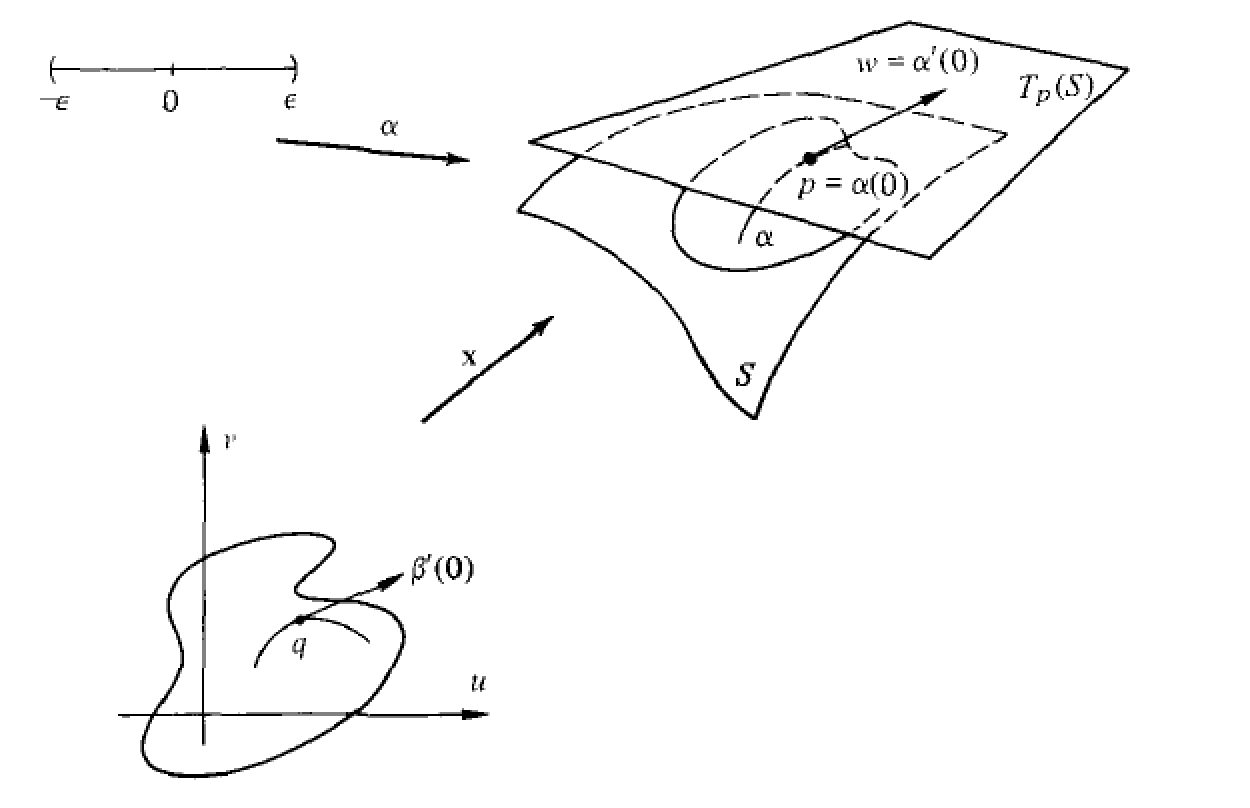
\includegraphics[scale = 0.5]{tangent_plane.png}}
\end{minipage}
\caption{\scriptsize
\textbf{The tangent plane as the subspace of tangent vector of embedded curves. Find the coordinate of the tangent vector in tangent space.}}
\end{figure}

\item \begin{definition}
The \emph{\textbf{differential}} of a map $\varphi: V\subset \cS_{1} \rightarrow \cS_{2}$ at $p\in \cS_{1}$ is a linear map $d\varphi_{p}: T_{p}S_{1} \rightarrow T_{\varphi(p)}S_{2}$, where $d\varphi_{p}(\mb{w}) = \beta'(0)$ for $\mb{w}\in T_{p}S_{1}$ with the curve on $\cS_{2}$ as $\beta = \varphi\circ \alpha$ and $\alpha: (-\epsilon, \epsilon) \rightarrow V$ is the curve on $\cS_{1}$. 
\end{definition}

\item \begin{proposition}\label{prop: tang_param}
Let $\mb{x}: U\subset \bR^{2} \rightarrow \cS$ be a parameterization of a regular surface $\cS$ and let $q\in U$. The \textbf{tangent plane} to $\cS$ at $\mb{x}(q)$ is given as 
\begin{align*}
d\mb{x}_{q}\paren{\bR^{2}} \subset \bR^{3}
\end{align*} as a $2-$dimensional linear subspace.
\end{proposition}  By the above proposition, the plane $d\mb{x}_{q}\paren{\bR^{2}}$, which passes through $\mb{x}(q) = p$, does not depend on the parametrization $\mb{x}$. 

\item (\emph{\textbf{Tangent vector via basis}})\\
 For $\alpha'(0)\equiv \mb{w} \in T_{p}S$, for some $\alpha = \mb{x}\circ  \beta$, where $\beta: (-\epsilon, \epsilon) \rightarrow U$ by $\beta(t) = (u(t), v(t))$, with $\beta(0) = q = \mb{x}^{-1}(p)$. Then 
\begin{align}
\alpha'(0)&= \frac{d}{dt}(\mb{x}\circ \beta)(0) = \frac{d}{dt}\mb{x}(u(t), v(t))(0)\\
&=\mb{x}_{u}u'(0) + \mb{x}_{v}v'(0) \label{eqn: tangent_line_coord}
\end{align} 
Thus under the basis $(\mb{x}_{u}, \mb{x}_{v})$ of $T_{p}S$, the coordinate of $\mb{w}$ in $T_{p}S$ is $(u'(0), v'(0))$, and $\mb{w}$ is the velocity of  the curve $\alpha$ is represented as $(u(t), v(t))$ in parameterization $\mb{x}$ at $t=0$. 

\item (\emph{\textbf{Differential of map via basis}})\\
 If $\mb{w} = (u'(0), v'(0))$ in $T_{p}(S_{1})$,  and $\varphi(u,v) = (\varphi_{1}(u,v), \varphi_{2}(u,v))$, with $\alpha(t) = (u(t), v(t))$, then the tangent of $\beta$ at $\varphi(p)$ is given via the differential of map of $\mb{w}$ at $p$ is given in its own coordinates as 
\begin{align}
 \beta'(0)= d\varphi_{p}(\mb{w}) &= \brac{\begin{array}{cc}
 \dpartdiff{\varphi_{1}}{u} & \dpartdiff{\varphi_{1}}{v} \\ 
 \dpartdiff{\varphi_{2}}{u} & \dpartdiff{\varphi_{2}}{v}
 \end{array} } \brac{\begin{array}{c}
 u'(0) \\ 
 v'(0)
 \end{array} } \label{eqn: diff_map_coord}
\end{align}
Thus $d\varphi_{p}$ as a linear mapping under coordinates $(\mb{x}_{u}, \mb{x}_{v})$ in $T_{p}S$ and $(\mb{x}^{'}_{u'}, \mb{x}^{'}_{v'})$ in $T_{p}S$ is given as the matrix $\brac{\begin{array}{cc}
 \partdiff{\varphi_{1}}{u} & \partdiff{\varphi_{1}}{v} \\ 
 \partdiff{\varphi_{2}}{u} & \partdiff{\varphi_{2}}{v}
 \end{array} } $.

\item \begin{definition}
A map $\varphi: U\subset \cS_{1} \rightarrow \cS_{2}$ is a \emph{\textbf{local diffeomorphism}} at $p\in U$ if there exists a neighborhood $V\subset U$ of $p$ such that $\phi$ restricted on $V$ is a diffeomorphism onto an open subset $\varphi(V)\subset \cS_{2}. $ 
\end{definition}


\item 
\begin{theorem}
If $\cS_{1}$ and $\cS_{2}$ are two regular surfaces and $\varphi: U\subset \cS_{1} \rightarrow \cS_{2}$ is a differentiable mapping of an open subset $U\subset \cS_{1}$ such that the differential $d\varphi_{p}$ of $\varphi$ at $p$ is an isomorphism, then $\varphi$ is a \textbf{local diffeomorphism} at $p$.
\end{theorem}


\item \begin{definition}
The (unit)  vectors that are normal to the tangent plane at $p$ is called \emph{the (unit) \textbf{normal vectors}} at $p$, denoted as $N(p)$.  It can be defined by the rule
\begin{align*}
N(p) &= \frac{\mb{x}_{u} \wedge \mb{x}_{v}}{\abs{\mb{x}_{u} \wedge \mb{x}_{v}}}(p)
\end{align*}
\end{definition}

\item The angle between two surfaces $\cS_{1}$ and $\cS_{2}$ at the intersecting point $p$ is defined as the angle btw two tangent plane at $p$ or the angle btw the normal vectors at $p$.

\end{itemize}

\subsection{The First Fundamental Form and Area}
\begin{itemize}
\item  The \emph{inner product} $\inn{\cdot}{\cdot}$ on the tangent space $T_{p}S$ is induced from $\bR^{3}$. 

\item \begin{definition}
 The \underline{\emph{\textbf{first fundamental form}}} of a regular surface $\cS\subset \bR^{3}$ at $p\in \cS$ is defined as a  \textbf{quadratic form},  $I_{p}: T_{p}S \rightarrow \bR$ given by 
\begin{align}
I_{p}(\mb{w}) &= \inn{w}{w}_{p} = \norm{w}{2}^{2} \ge 0\; \; \mb{w}\in T_{p}S. \label{eqn: first_fund_form1}
\end{align}
\end{definition}

\item For orthogonal basis $\set{\mb{x}_{u}, \mb{x}_{v}}$, the first fundamental form is the \emph{\textbf{Pythagorean theorem}} in $\cS$. 

\item (\emph{\textbf{The first fundamental form via basis}})\\
Under the basis $\set{\mb{x}_{u}, \mb{x}_{v}}$ associated with $\mb{x}(u,v)$ at $p$, the first fundamental form can be formulated explicitly. Since $\mb{w} = \alpha'(0)$ for $\alpha:  (-\epsilon, \epsilon) \rightarrow \cS$ with $\alpha(t) = (u(t), v(t))$ and $p = \alpha(0) = \mb{x}(u(0), v(0))$, thus
\begin{align}
I_{p}(\alpha'(0)) &= \inn{\mb{x}_{u}u'(0) + \mb{x}_{v}v'(0)}{\mb{x}_{u}u'(0) + \mb{x}_{v}v'(0)} \nonumber\\
&= \inn{\mb{x}_{u}}{\mb{x}_{u}}\paren{u'(0)}^{2} + 2\,\inn{\mb{x}_{u}}{\mb{x}_{v}}\paren{u'(0)v'(0)} +  \inn{\mb{x}_{v}}{\mb{x}_{v}}\paren{v'(0)}^{2}\nonumber\\
&= E\,\paren{u'(0)}^{2} + 2\,F\paren{u'(0)v'(0)} + G\paren{v'(0)}^{2} \label{eqn: first_fund_form2}
\end{align}
and 
\begin{align}
E(u(0), v(0)) &= \inn{\mb{x}_{u}}{\mb{x}_{u}}_{p}\nonumber\\
F(u(0), v(0)) &= \inn{\mb{x}_{u}}{\mb{x}_{v}}_{p}\nonumber\\
G(u(0), v(0)) &= \inn{\mb{x}_{v}}{\mb{x}_{v}}_{p} \label{eqn: first_fund_coeff}
\end{align} are \emph{\textbf{coefficients of the first fundamental form}} in the basis $\set{\mb{x}_{u}, \mb{x}_{v}}$. Note that $p=\mb{x}(u,v)$ runs in the coordinate neighborhood, the quantities $E(u,v), F(u,v), G(u,v)$ are differentiable function on $U$.

\item Also, we can compute the angle btw two parameterized regular curve $\alpha(t)$ and $\beta(t)$ on $\cS$ that intersects at $t=t_{0}$ as 
\begin{align*}
\cos(\theta) &= \frac{\inn{\alpha'(t_{0})}{\beta'(t_{0})}}{\norm{\alpha'(t_{0})}{2}\,\norm{\beta'(t_{0})}{2}}.
\end{align*}
Then the angle $\phi$ btw two coordinate curves of a parameterization $\mb{x}(u,v)$ is given by 
\begin{align}
\cos(\phi) &= \frac{\inn{\mb{x}_{u}}{\mb{x}_{v}}}{\norm{\mb{x}_{u}}{2}\,\norm{\mb{x}_{v}}{2}} = \frac{F}{\sqrt{E\,G}}. \label{eqn: first_fund_angle_basis}
\end{align}
It follows that the coordinate curves of a parametrization are \emph{orthogonal} if and only if $F(u, v)  = 0$ for all $(u, v)$. Such a parametrization is called an \textbf{\emph{orthogonal parametrization}}.


\item The \textbf{matrix} of first fundamental form is given as 
\begin{align}
\mb{J}\equiv \brac{\begin{array}{cc}
\inn{\mb{x}_{u}}{\mb{x}_{u}}_{p} &  \inn{\mb{x}_{u}}{\mb{x}_{v}}_{p} \\ 
 \inn{\mb{x}_{v}}{\mb{x}_{u}}_{p} & \inn{\mb{x}_{v}}{\mb{x}_{v}}_{p}
\end{array} } = 
\brac{\begin{array}{cc}
E & F \\ 
F & G
\end{array} } \label{eqn: first_fund_form3}
\end{align}
and for $\mb{w} = \alpha'(0) = (u'(0), v'(0))$, 
\begin{align*}
I_{p}(\mb{w}) &= \mb{w}^{T}\,\mb{J}\,\mb{w}
\end{align*}

\item Given the first fundamental form $I(\alpha'(t))$ on $T_{p}S$, we can evaluate the the \textbf{arc length} without using its coordinate in $\bR^{3}$ 
\begin{align}
s &= \int_{0}^{t} \sqrt{I(\alpha'(t))}  dt\nonumber\\
&= \int_{0}^{t} \sqrt{E(u'(t))^{2}+ 2\,F\,(u'(t)v'(t)) + G\,(v'(t))^{2}  }  dt \nonumber\\
&=  \int_{0}^{t} \sqrt{ \dpartdiff{\mb{\alpha}}{t}^{T}\mb{J}\, \dpartdiff{\mb{\alpha}}{t} }  dt  \label{eqn: arc_leng_2}
\end{align}

\item Another metric question that can be treated by the first fundamental form is the computation (or definition) of the \emph{area} of a bounded region of a regular surface $\cS$. 

\begin{definition}
A \emph{\textbf{(regular) domain}} of $\cS$ is an \emph{\textbf{open}} and \emph{\textbf{connected}} subset of $\cS$ such that its \emph{\textbf{\textbf{boundary}}} is the image in $\cS$ of a circle by a \emph{differentiable} \emph{homeomorphism} which is regular (that is, its \emph{differential} is nonzero) except at a finite number of points. A \emph{\textbf{region}} of $\cS$ is the union of a domain with its boundary. 
A region of $\cS \subset \bR^3$ is \emph{\textbf{bounded}} if it is contained in some ball of $\bR^3$.
\end{definition}

\item \begin{definition}
Let $\cR \subset \cS$ be a \emph{bounded region} of a regular surface contained in the coordinate neighborhood of the parametrization $\mb{x}: U \subset \bR^2 \rightarrow \cS$. The positive number
\begin{align}
\int\int_{Q} \abs{\mb{x}_{u}\wedge \mb{x}_{v}}dudv, \quad Q = \mb{x}^{-1}(\cR) \label{eqn: area_first_fund}
\end{align} 
is called the \emph{\textbf{area}} of $\cR$. Here $\abs{\mb{x}_{u}\wedge \mb{x}_{v}} = \sqrt{EG - F^{2}}$.
\end{definition}
\end{itemize}




\newpage

\section{Examples and exercises}
\subsection{Curves}

\subsection{Surfaces}

\newpage
\bibliographystyle{plainnat}
\bibliography{book_reference.bib}
\end{document}